
%%% Local Variables:
%%% mode: latex
%%% TeX-master: t
%%% End:

\chapter{引言}
\label{chap:intro}

互联网应用如电子邮件、搜索、网络购物、社交网络、在线视频、网络地图等, 已经成为人们
生活的一部分。这些应用往往要为上亿用户服务,意味着互联网应用已变成如电力一样的社会
公共服务,而支撑拥有海量用户互联网应用的数据中心也成为如同发电厂一样的社会核心基础
设施。

长尾延迟(Tail Latency)问题在数据中心中受到越来越多的关注,造成长尾延迟的原因有很
多,其中最为重要的原因就是资源共享带来的干扰。
由于没有行之有效的方案对干扰进行控制,目前典型的数据中心都使用隔离的方式来减小干扰,
这一方案虽然有效缓解了长尾延迟,但它也带来了资源利用率过低的问题,
现有商用数据中心的资源利用率普遍只有10\%-30\%左右,造成极大的浪费。
如何解决服务质量与资源利用率的问题是当前业界面临的重大挑战。

本章内容安排如下:首先介绍新计算模式对数据中心的挑战,然后讨论现有数据中心技术的局
限性,即服务质量与资源利率冲突的原因,进而提出一种面向数据中心应用服务质量保障的
体系结构,最后将阐述本文的研究动机,介绍本文的主要贡献和组织结构。

%服务质量(QoS)与资源利用率是数据中心运营时需要考虑的两个重要指标,前者严重影响用户
%体验,而后者直接与数据中心的运营成本相关。然而现有的计算机体系结构并没有为服务质量
%保障提供足够的支持,造成这两个指标在现实状况下存在冲突。为了保障用户体验,在实际系
%统部署时,会更多的考虑服务质量这一指标,造成数据中心的资源利用率严重低下,普遍只有
%10\%-30\%左右。基于这一现状,本文主要讨论如何设计一种高效的数据中心体系结构,使得
%数据中心在保障应用服务质量基础上,达到较高的资源利用率。
%

\section{新计算模式对数据中心的挑战}

\subsection*{计算模式1:以云计算为基础的移动计算}

随着移动设备(平板电脑、智能手机)计算能力不断增强、成本不断降低以及无线通信技术的
快速发展,移动计算时代已经来临。如表\ref{tab:ganter-sales}所示,
Gartner调研数据显示平板电脑和手机(包含智能手机和普通手机)销量不断增加,
与此同时PC销量则不断下降。
而IDC预测到2015年智能手机销量将超过14亿部,占所有个人计算设备(包括PC、平板电脑和智能手机等)69\%的销量份额。

% Gartner关于电脑与移动设备销量的统计 
\begin{table}[htb]
  \centering
  \begin{minipage}[t]{0.9\linewidth}
  \caption[全球个人计算设备市场销量统计]{全球个人计算设备市场销量统计(单位:千部)}
  \label{tab:ganter-sales}
    \begin{tabular*}{\linewidth}{lrrrrr}
      \toprule[1.5pt]
      {\heiti 设备类型} & {\heiti 2012年} & {\heiti 2013年} & {\heiti 2014年} & {\heiti 2015年} & {\heiti 2016年} \\
      \midrule[1pt]
      PC(台式机、笔记本) &   341,273 &   296,131 &   279,000 &   259,000 &   248,000 \\ 
      超级本               &     9,787 &    21,517 &    39,000 &    62,000 &    85,000 \\ 
      平板电脑             &   120,203 &   206,807 &   216,000 &   233,000 &   259,000 \\ 
      手机                 & 1,746,177 & 1,806,964 & 1,838,000 & 1,906,000 & 1,969,000 \\ 
      其它移动设备         &       --- &     2,981 &     6,000 &     9,000 &    11,000 \\
      %总计                 & 2,217,440 & 2,334,400 & 2,378,000 & 2,470,000 & 2,572,000 \\
      \bottomrule[1.5pt]
    \end{tabular*}\\[2pt]
    \footnotesize
    数据来源:Gartner,2012年(http://www.gartner.com/newsroom/id/2610015),
    2013年(http://www.gartner.com-\\/newsroom/id/2791017),
    2014-2016年(http://www.gartner.com/newsroom/id/2954317)
  \end{minipage}
\end{table}

移动计算的快速发展带来新的计算模式:移动设备通过无线通信与运行在云计算平台的各类应
用服务进行交互。据可靠消息,目前一些主要的互联网公司(如Facebook和Baidu等)均表示,
来自移动设备的请求已占到40\%以上,并且仍在快速增长,很快将超过PC。随着4G时代的到来,
这种移动计算模式将成为未来的主流。

快速增长的移动计算需求对云计算平台的核心——数据中心带来了严峻的挑战。这种交互式计算
模式,快速的服务响应时间是衡量服务质量(Quality-of-Service,QoS)的关键指标,是让用
户满意、留住用户的关键。有研究表明,如果服务响应时间增加,公司收入就会减少。
例如,2009年微软在Bing搜索引擎上也开展实验,发现当服务响应时间增加到2000ms时,
每个用户带给企业的收益更是下降了4.3\%。由于该实验对公司产生了负面影响,最终不得不被
终止[8]。Amazon也发现其主页加载时间每增加100ms就会导致销售额下降1\% 。而Google更是
发现当搜索结果返回时间从0.4s增加到0.9s时,广告收入下降了20\%。

\begin{figure}
\begin{minipage}{0.48\textwidth}
  \centering
  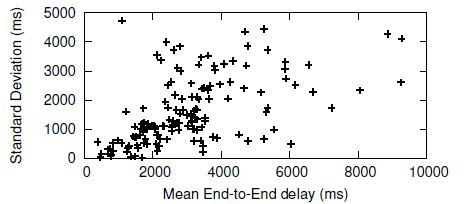
\includegraphics[height=5cm]{intro/end2end-delay}
  \caption[北美移动应用用户感知时延分布]{北美移动应用用户感知时延分布:平均延迟超过2秒且具有很大的波动性}
  \label{fig:end2end-delay}
\end{minipage}\hfill
\begin{minipage}{0.48\textwidth}
  \centering
  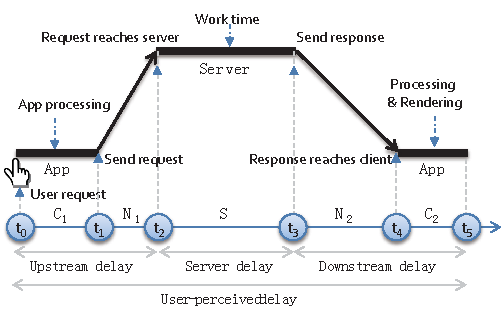
\includegraphics[height=5cm]{intro/interact-apps}
  \caption[一个典型的交互式请求的5个阶段]{一个典型的交互式请求的5个阶段:C1->N1->S->N2->C2 \cite{timecard2013}}
  \label{fig:interact-apps}
\end{minipage}
\end{figure}

移动计算的响应时间仍然存在很大的提升空间。
如图\ref{fig:end2end-delay}所示,微软公司实验数据表明在北美网络环境下,
交互式移动设备的平均时延超过2秒,而且存在较大的波动性。
图\ref{fig:interact-apps}显示典型移动交互式应用的用户请求时延分为5个阶段,
最近研究\cite{timecard2013}表明其中数据中心服务器的处理时延S约为1.2秒,占60\%。
随着4G网络的来临,数据中心将面临更大规模用户数据的处理请求。
因此,如何快速处理和及时响应移动计算请求将成为数据中心设计的核心目标之一。


\subsection*{计算模式2:面向大数据处理的实时计算}

大数据时代的到来使大数据处理架构受到越来越多的关注。2013年底中国计算机学会(CCF)
大数据专家委员会发布的《2014年大数据发展趋势十大预测》 报告中,来自学术界、产业界、
海外、跨界特邀和政府的122位专家们普遍认为,Hadoop/MapReduce框架一统天下的模式将被
打破,而实时流计算、分布式内存计算、图计算框架等将并存。

\begin{figure}[H]
  \centering
  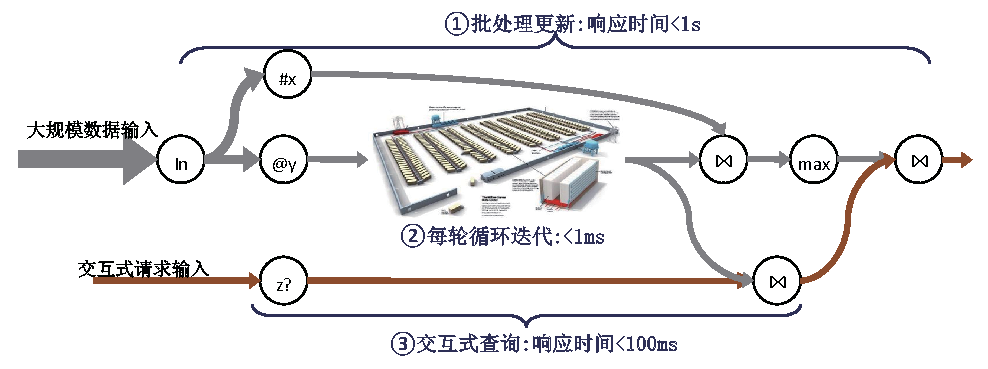
\includegraphics[height=6cm]{intro/batch-apps}
  \caption{典型的3类大数据处理需求以及相应的响应时间要求}
  \label{fig:batch-apps}
\end{figure}


大数据处理对数据中心和处理架构提出新的挑战,图\ref{fig:batch-apps}显示了典型的
大数据处理需求:首先需要支持数据的批处理更新模式(<1s);
其次数据处理会分解为多次迭代计算(<1ms);
再次还要支持实时计算模式,处理多用户的交互式查询请求(<100ms);
而这些处理所需要的数据
存放在同一个数据中心。搜索引擎是一个典型的例子,既需要对大规模网页进行内容处理,
迭代计算页面的pagerank,还需要处理大量用户的关键字查询请求。

尽管大数据处理希望能将各种处理集成在一个处理架构上,然后部署在一个数据中心。但如果
实时计算与企业营收相关,比如搜索引擎、在线购物等在线服务应用,那么正如微软Bing实验
所示,这些面向在线服务应用的实时计算的服务质量就非常关键(以下用“在线应用”
代表“实时计算”)。为了保障在线应用的服务质量,主流互联网企业一般将在线应用与大规模
批处理作业分别部署到不同的数据中心,以减少批处理作业对在线应用的干扰。但由于用户查
询请求数量具有显著的随时间变化的波动性,这种分离作业、单独部署的模式会导致在线应用
数据中心的资源平均利用率很低。如图4所示,Google的两类数据中心CPU利用率相差达2.5倍,
在线应用数据中心资源利用率仍有很大提升空间。


%% 典型的数据中心一般有5~10万台服务器组成,建设与运行维护成本往往高达几十亿人民
%% 币。然而出于保障应用服务质量的原因,现有数据中心只能维持较低的资源利用率,导致大量
%% 资源浪费。因此,本项目总体研究目标为如何设计高效通用数据中心体系结构:“通用”表
%% 示数据中心可同时运行各种不同类型应用;“高效”表示数据中心能在保障延迟敏感应用的服
%% 务质量基础上,达到较高的资源利用率(CPU利用率>60\%)。
%% 
%% 典型的数据中心一般有5~10万台中低端服务器组成,这些服务器通过内部网络互连,一起协同
%% 运行互联网应用为海量用户服务。因为这类数据中心规模很大,往往部署在大型仓库级别的机
%% 房,从应用角度来看就如同一台计算机,因此也被称为
%% “仓库级计算机(Warehouse-Scale Computer)“ \cite{WSC}。
%% 国内外著名的互联网公司往往拥有多个数据中心,服务器数量达到数十万甚
%% 至上百万台。例如,谷歌(Google)的数据中心服务器数量已经超过百万台为全球用户提供
%% 搜索、邮件、地图等服务[2];亚马逊(Amazon)仅EC2就部署了约50万台服务器提供云计算服
%% 务[3];据可靠消息,国内腾讯公司也拥有约30万服务器为用户提供各种互联网服务。
%% 
%% 尽管目前互联网企业的数据中心已经颇具规模,但一个趋势是未来数据中心还将持续发展。一
%% 方面互联网用户数量仍在不断增长,目前全球已有24亿网络用户,但很多机构预测未来全球还
%% 将新增30亿网民融入到互联网[4],这会对数据中心的数量和规模都提出更多需求。另一方面快
%% 速发展的移动终端已超越个人计算机(PC),成为终端计算设备的主流。由于移动设备性能相对
%% 较低、存储容量较小,将计算与存储转移到数据中心的需求也变得越来越强烈。因此数据中心作
%% 为基础设施也会日益重要。


\section{现有数据中心技术的局限性}

通过上述分析可知,移动计算与实时计算均对快速响应用户请求提出了强烈的需求。而当前数
据中心为了保障用户请求的服务质量,不得不通过采用牺牲资源利用率、保留过量资源的方式。
Google的数据中心技术一直处于领先地位,我们以Google为例分析数据中心资源利用率现状。
图\ref{fig:google-util-2006}显示了2006年Google数据中心平均CPU利用率为30\%左右。
但到2013年,虽然Google将数据中心分为了两类,并且批处理数据中心已经能达到75\%的CPU利用率,
但在线应用数据中心仍停留在30\%。
我们对国内企业调研发现,几大主流互联网企业在线应用数据中心CPU利用率一般都低于20\%,
有的甚至低于10\%,仍然存在很大的提升空间。

% Google数据中心利用率 
\begin{figure}
\begin{minipage}{0.57\textwidth}
  \centering
  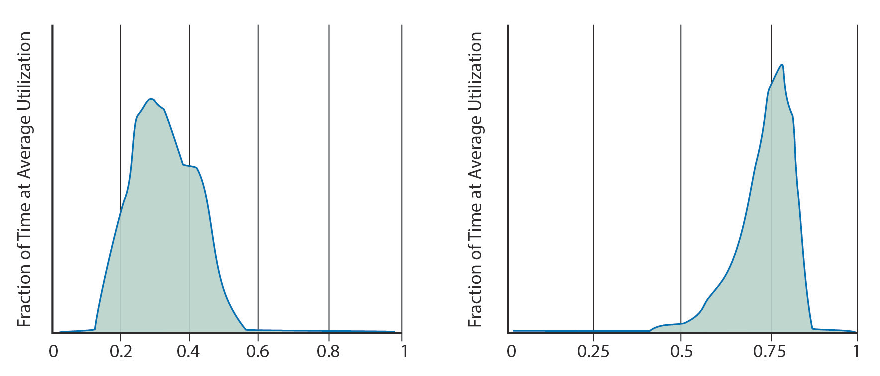
\includegraphics[height=4cm]{intro/google-util-2013}
  \caption[Google数据中心CPU利用率分布(2013年)]
    {Google数据显示2013年1至3月在线应用数据中心CPU利用率平均只有30\%(左图),
     而批处理作业数据中心则能达到75\%的利用率(两个数据中心均为2万台服务器)}
  \label{fig:google-util-2013}
\end{minipage}\hfill
\begin{minipage}{0.39\textwidth}
  \centering
  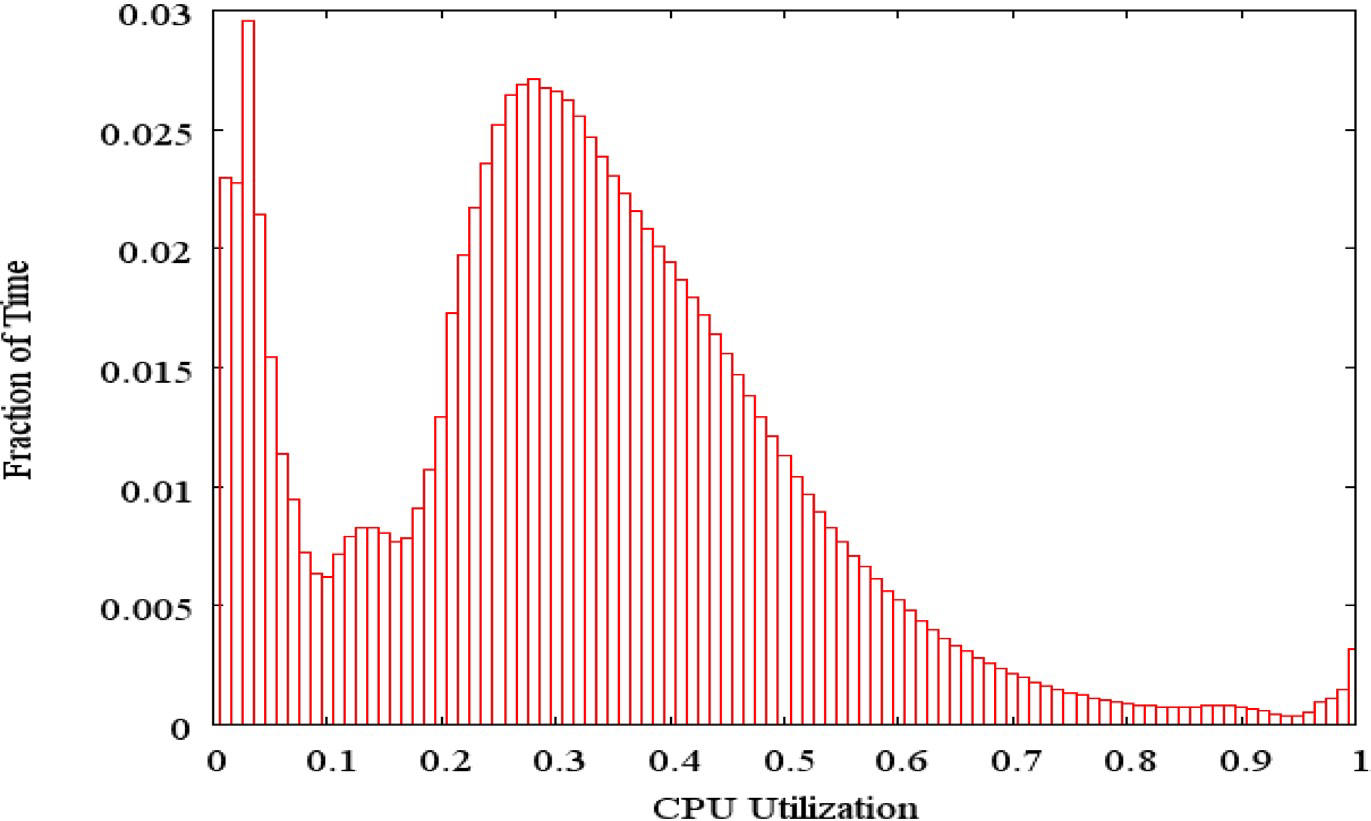
\includegraphics[height=3.5cm]{intro/google-util-2006}
  \caption[Google数据中心CPU利用率分布(2006年)]
    {Google在2006年数据中心(5000台服务器)6个月的CPU利用率分布}
  \label{fig:google-util-2006}
\end{minipage}
\end{figure}

尽管在线数据中心资源利用率只有30\%,但Google已经观察到严峻的长尾延迟现象---最慢的
1\%~10\%请求处理时间远大于所有请求的平均响应时间。
如图6所示,Google某后台服务延迟响应时间平均仅为5~6ms,但是却有相当一部分请求响应时间
超过了100ms[49]。而长尾延迟现象在数据中心环境下会被更进一步放大,因为一个用户请求需要
几百上千台服务器共同完成,只要有一台服务器的处理速度受到干扰,就会导致整个请求的处理
时间增加。Google的Jeff Dean在2012年Berkeley的报告[11]中就指出了长尾现象的严重性,假设
一台机器处理请求的平均响应时间为1ms,有1\%的请求为长尾处理时间会大于1s 
(99th-Percentile)。如果一个请求需要由100个这样的节点一起处理,那么就会出现63\%的请求
响应时间大于1s(如图7所示)。

造成在线应用数据中心资源利用率低和长尾延迟现象的核心原因是现有数据中心技术无法在多
应用混合运行时消除应用间干扰,以实现不同应用之间的性能隔离。
Google的Jeff Dean与Luiz Barroso在2013年2月的《Communication of the ACM》上撰文
“The Tail at Scale”[10]分析确认导致长尾延迟的首要原因就是资源共享,
包括体系结构层次的CPU核、Cache、访存带宽、网络带宽等,而干扰不仅来自应用,
还会来自系统软件层次的后台守护作业、监控作业、共享文件系统等。
Google在分布式架构和软件层次采用了多种缓解长尾延迟的技术,
包括操作系统容器隔离技术[12]、应用优先级管理[13]、备份请求[11]、同步后台管理进程[11]等,
取得了一定的效果,但却无法消除硬件体系结构层次上的应用之间的干扰,
导致仍然会出现图6这样的长尾延迟。

因此,现有数据中心处于“无管理的资源共享”状态,这
导致出现资源利用率与应用服务质量之间的矛盾:
一方面通过多个应用同时在数据中心部署实现资源共享能有效提高资源利用率,
但另一方面多个应用共享资源又会出现相互干扰严重影响应用的服务质量。
因此,目前企业不得不采用预留额外资源以保障延迟敏感的在线应用服务质量,
这导致很低的数据中心利用率。
而且随着多核技术的发展,单个服务器内的资源越来越多,
其上混合部署的应用数目也在不断增加,更会加剧这种矛盾。


\section{本文的研究动机}

现有数据中心技术面临资源利用率与应用服务质量的矛盾,其根本原因是大量数据中心共享资源
属于“无管理共享”状态。要实现高效通用数据中心目标,核心是从硬件上改变资源的“无
管理共享”现状以实现在体系结构上支持应用服务质量保障,在此基础上实现数据中心资源根据应
用动态管理以提高资源利用率。

回顾历史,当前数据中心面临的问题与1990年代的Internet具有相似之处。
当时流媒体、电子商务、电子邮件和FTP等大量网络应用的兴起,它们具有不同的QoS需求。
为了在IP网络中为这些应用提供端到端的服务质量保障,
互联网工程任务组(Internet Engineering Task Force, IETF)于1998年提出了区分化服务
(Differentiated Services)的概念。而如今,区分化服务已经成为应用最广泛的服务质量保障
机制之一。该技术的核心是在IP包头中定义长度为8-bit的区分化服务域,用以表示应用的
服务质量分类标识,因此路由器、交换机等网络设备便可以使用该信息对不同类别的数据包
进行区分处理,以达到区分化服务的目的。
软件定义网络(SDN)的出现,进一步促进了网络领域服务质量保障的发展,
其主要原理可以概括为:(1) 控制平面与数据平面分离;(2)集中控制的统一编程接口。

同时,计算机内部也可以被看做一个网络,如图\ref{fig:computer-as-a-network}所示,
CPU核、共享缓存、内存控制器、I/O设备等可以被看做是网络节点;除了处理请求以外,
这些“网络节点”与网络中的路由器/交换机具有相似的请求转发功能;
而它们之间也通过包进行通信,如:片内通信使用NoC包,片间通信的QPI/HT包,
以及I/O部分使用的PCI-E包。
将网络领域的区分化服务和软件定义网络的思想应用到计算机内部的网络,
用以解决数据中心当前面临的资源利用率与应用服务质量矛盾,是本文的主要研究思路与动机。

与在网络中部署SDN相比,在计算机体系结构“网络”中部署SDN会面临以下三个挑战:

First, in a network, usually the network stack is the only source
for generating packets so it is easy to add tagging mechanism into
the network stack. In a computer, in contrast, a number of different
hardware components can generate different types of packets.
Thus, we need to address how to tagging packets generated by various
hardware components. (x4.1)

Second, unlike network routers that perform almost the same
store-and-forward behavior, hardware components in a computer
behave differently. It is challenging to figure out a uniform control
plane structure for different hardware components such as LLC,
memory and I/O devices. (x4.2)

Finally, there is already a firmware running in a network router
for users to access and configure the router’s control plane. However,
conventional computers lack similar firmware. The current
IPMI2 [6] firmware in servers only performs limited monitoring
and management functionality such as temperature, fan speed and
power. Thus, it is essential to devise a firmware that provides a uniform
interface for server operators to access control planes of hardware
components. Moreover, a flexible programming methodology
is desirable as well (x5).



%本项目总体研究目标是研究新型高效通用数据中心体系结构,能在保障应用服务质量
%的基础上将数据中心计算资源利用率提高到60\%以上。从技术挑战来看,计算机资源管理亟需新的
%具有以下特征的技术架构:
%(1)细粒度共享,有利于提高资源利用率;
%(2)性能隔离,有利于提高应用服务质量;
%(3)快速动态响应,有利于资源按需分配;
%(4)灵活协同配置,有利于协同多种资源配置以适应多种应用场景。


\section{论文的主要工作}

本研究的目的是通过对真实环境、真实应用的访存行为特征进行更全面细致的分
析,
探索服务质量保障的体系结构支持,
内存系统影响计算机整体性能的更深层次的原因,从而为体系结构、系统软件
等的设计与优化提供一些建议。
论文的主要工作围绕上述三个阶段开展1:


\section{论文的主要贡献}
aaa


\section{论文的组织结构}

本文共分八章,第一章介绍移动计算带来的新计算模式对数据中心的挑战,然后讨论现有
数据中心技术的局限性,并针对现有体系结构提出了新的需求,最后介绍了论文的研究动机、
主要贡献和组织结构。

第二章介绍体系结构领域解决服务质量问题的现有研究,并对比以网络领域的相关内容,
讨论两者相互借鉴的可能性。

第三章对现有体系结构的服务质量支持进行评估,包括软件(cgroup, hyperviso)和硬件
两个层次。

第四章介绍资源管理可编程体系结构的概念与核心思路,并将其映射到现有体系结构,
讨论其可行性。同时应用资源管理可编程体系结构实现全硬件虚拟化,并讨论其关键技术。

第五章讨论模拟器实现,主要从功能设计角度对控制面设计,与资源管理可编程实现,
硬件支持、Trigger-Action机制,模拟的方式验证PARD的有效性。

第六章基于前两章的设计给出本文资源管理可编程体系结构的FPGA原型系统实现,
并对原型系统各部分功能的正确性、性能与开销进行了详细评测。

第七章在数据中心场景下,对本文资源管理可编程体系结构在分布式场景下应用进行讨论。

第八章总结全文并介绍未来可能的研究工作。

